\subsection{Diagrammi dei package}
\begin{figure}[hb]
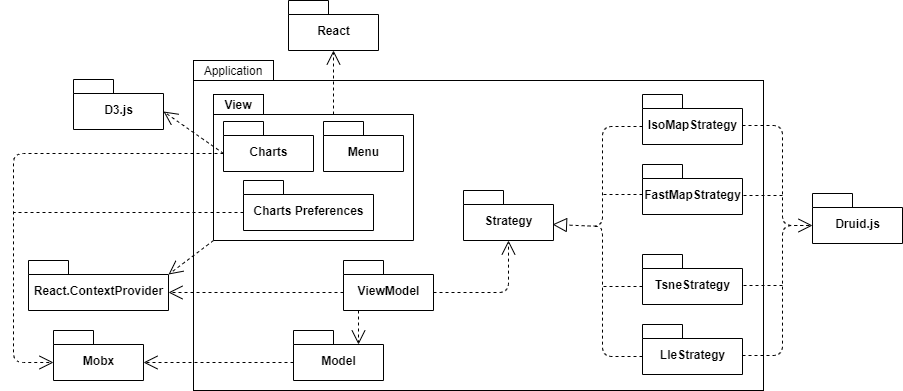
\includegraphics[width=15.8cm]{Images/Allegato Tecnico-Package}
\centering
\caption{Diagramma dei package client side}
\end{figure}

Il diagramma sopra riportato descrive a livello di package le parti che compongono il lato client dell'applicazione. In particolare si può notare che:
\begin{itemize}
	\item \textit{View} e \textit{Model} non siano direttamente collegati, ma il passaggio delle informazioni avviene attraverso il \textit{ViewModel} e il componente \glo{\textit{Context Provider}} fornito da React;
	\item MobX ha il ruolo fondamentale di applicare l'Oberserver design pattern, ossia rendere i dati contenuti nel \textit{Model} observable e i componenti della vista che li utilizzano (grafici e form per la loro personalizzazione) observer;
	\item Druid.js è importata nelle classi per eseguire la riduzione dimensionale e D3.js solo nei componenti della vista dedicati all'implementazione delle varie visualizzazioni.
\end{itemize}  %componente fornito da React per consumare il contesto creato



%\begin{figure}[hb]
%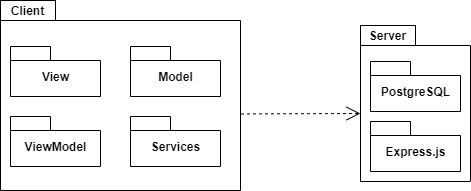
\includegraphics[width=15.8cm]{Images/Allegato Tecnico-Package 2}
%\centering
%\caption{Connessione tra client side e server side}
%\end{figure}
